%!TEX root = ../thesis.tex
\chapter{Entropy rate estimation}\label{ch:crossentropy}

\epigraph{\em ``Semantic aspects of communication are irrelevant to the engineering problem.''}{Claude Shannon, {\em A Mathematical Theory of Communication}, 1948}

Extracting information flows is a problem deeply rooted in information theory. To examine these flows requires tools to quantify and measure this information in the form of natural language. As discussed in \autoref{ch:background}, the words used to construct language have no qualitative meaning in the context of the numerical analysis. Thus the tools are comparative in nature. Indeed, information theory has been used extensively to compare properties of information in language~\cite{shannon_prediction_1951,cover_convergent_1978,brown_estimate_1992}. 

In this chapter, we extend this philosophy in two key ways. We introduce a non-parametric entropy rate estimator and check its assumptions using real data. We then generalise this entropy rate to a cross entropy rate, developing a tool for analysing information flows. These new estimators are then made into a high speed open-source package which is applied to our news data. 

\section{Entropy rate estimation}

Recall \autoref{def:entropyrate} of the entropy rate of a stochastic process. While a useful theoretical tool, this can be very difficult to compute, requiring knowledge of the joint entropy for an infinite set of realisations.

To overcome this, we seek a way to estimate the entropy of the process from a known sequence of data. In 1998 Kontoyiannis \emph{et al.}~\cite{kontoyiannis_nonparametric_1998} proved the convergence of a non-parametric entropy estimator for stationary processes.

\begin{definition}[Kontoyiannis Entropy Rate] \label{def:Kontoyiannis}
	For a discrete valued stochastic process $\mathcal{X} = \{X_i\}_{i=0}^N$, with $N$ realisations, the entropy rate is given by,
	\begin{equation}\label{eq:entropy:Kontoyiannisdef}
		H(\mathcal{X}) = \lim_{N\to \infty}\frac{N \log N }{\sum_{i=0}^N \Lambda_{i} },
	\end{equation}
	where  $\Lambda_{i}$ is the length of the shortest subsequence starting at position $i$ that does not appear as a contiguous subsequence in the previous $i$ symbols, $X_{0}^{i} = \{X_k\}_{k=0}^i $. This can also be obtained by adding 1 to the longest match-length, 
	 \begin{equation}\label{eq:entropy:lambda}
	  \Lambda_{i}=1+\max \left\{\ell: X_{i}^{i+\ell}=X_{j}^{j+\ell}, 0 \leq j \leq N-i, 0 \leq \ell \leq N - i - j \right\}.
	 \end{equation}
\end{definition}

%<lit review>
This idea of using matched sub-sequences of text draws from the original work by Lempel and Ziv~\cite{ziv_universal_1977} in compression algorithms. These algorithms attempt to compress a sequence down into the smallest possible representation, which at perfect efficiency would be the entropy, $H$. However these universal coding algorithms have no universal rate of convergence~\cite{shields_universal_1993, shields_universal_1995} and in practice other approaches are often employed, tailored to the specific application at hand.

The idea of an entropy estimator based on match lengths was originally put forward by Grassberger~\cite{grassberger_estimating_1989} and proved consistent for independent and identically distributed (i.i.d.) processes and mixing Markov chains~\cite{shields_entropy_1992}, stationary processes~\cite{kontoyiannis_prefixes_1994} and more generally for random fields~\cite{quas_entropy_1999}.


Wyner and Ziv~\cite{wyner_asymptotic_1989} showed that for every ergodic process the match length $\Lambda_{n}$ grows like $\frac{\log{n}}{H}$ in probability.  Extending from this notion Kontoyiannis \emph{et al.} showed the convergence of \autoref{eq:entropy:Kontoyiannisdef} in stationary ergodic processes using the match-length $ \Lambda_{i}$. This match-length in \autoref{eq:entropy:lambda} can be seen as the length of the next phrase to be encoded in the sliding-window Lempel–Ziv algorithm.

%<match lengths>
Conceptually, this match-length is simple. \autoref{fig:entropy:matchlength} shows the calculation of two match-lengths at different time points of a line from Green Eggs and Ham by Doctor Seuss. At each index $i$, the elements immediately proceeding ($i, i+1, i+2, \dots$) are compared to the history of elements before $i$. The matches of length $k$ are found such that the elements from $j$ to $j+k$ perfectly match the elements from $i$ to $i+k$, for any $j<i$ where $k$ is then maximised. This search only considers the length of the match, regardless of its location in the history. 

\begin{figure}[!htbp]
	\centering
	\includestandalone[width=\textwidth]{chapter2/figs/tikz/lambda_count}
	\caption{An example calculation of the match-length based $\Lambda_i$ applied to a words in a line of text from Green Eggs and Ham by Doctor Seuss. The {\color{blue}blue texts} are words which have been matched from past to the future. As $i$ changes, the longest match length possible starting at index $i$ will change.\label{fig:entropy:matchlength}} 
\end{figure}
%</match lengths>

Even before its formalisation by Kontoyiannis \emph{et al.}, similar estimators had appeared in the literature applied to experimental data to determine the entropy rates of processes~\cite{chen_using_1993, chen_fast_1995, farach_entropy_1995, juola_what_1997}.
%</lit review>

% Final note
Moving forward we will assume any any discussion of the \emph{entropy rate} of a single process is assumed to be the \emph{Kontoyiannis entropy rate} of that process, unless otherwise stated.


% ASSSUMPTIONS
\section{Assumptions of entropy rate estimation}

The proof of convergence of this entropy rate places some limits on the process of investigation. In particular, three assumptions are made for convergence: ergodicity, stationarity and the Doeblin Condition (DC).

The Doeblin Condition is a reasonably weak condition, but is fundamental in the proof of the convergence. Simply put, the DC requires that after an arbitrary $r$ time steps, every state is possible again with positive probability~\cite{kontoyiannis_prefixes_1994}. More formally, the definition is as follows.

\begin{definition}[Doeblin Condition (DC)]
	There exists an integer $r\geq 1$ and a real number $\beta \in(0,1)$ such that, for all states $x_{0} \in \mathcal{A}$, 
	$$P\left\{X_{0}=x_{0} \mid X_{-\infty}^{-r}\right\} \geq \beta, $$ 
	with probability one. 
\end{definition}

Fortunately, as Kontoyiannis \emph{et al.} themselves state, the DC is ``certainly satisfied by natural languages''~\cite{kontoyiannis_nonparametric_1998}. 

In contrast, the assumptions of ergodicity and stationarity are  harder to confirm. A long-standing assumption of information theory is that natural language can be modelled by a stationary process~\cite{shannon_mathematical_1948, shannon_prediction_1951, cover_elements_2012}. The assumption, while flawed, has a long precedent and we use it again in this work.

Much of the literature including the work of Kontoyiannis assume ergodicity of natural language, however some suggest that language should be modelled by a \emph{strongly nonergodic} stationary process~\cite{debowski_is_2018}. In brief, this contention is founded upon the idea that any given collection of text, such as a book, has a topic containing a small finite subset of words. Which suggests that its text cannot explore the full state space of language. While well founded, our interest is not to look at the entropy rate of the English language as a whole, but rather to look at the entropy rate of individual text streams, which can all explore the state space of news under consideration. As such, the assumptions of ergodicity and stationarity appear justified in the context of the problem.


%<Convergence>
\subsubsection{Convergence}
With the assumptions of the proof addressed, the challenge of entropy rate estimation convergence needs to be examined. The entropy rate defined in \autoref{eq:entropy:Kontoyiannisdef} is based upon an infinite set of data. In reality, we have finite data, and need to examine the convergence of a modified estimator.

\begin{definition}[Kontoyiannis Entropy Rate Estimator] \label{def:Kontoyiannisestimate}
	The Kontoyiannis Entropy Rate in \autoref{def:Kontoyiannis} can be estimated on a finite stochastic process $\mathcal{X} = \{X_i\}$, with $N$ realisations, by
	\begin{equation}\label{eq:estimate}
		\hat{h} = \frac{N \log N }{\sum_{i=0}^n \Lambda_{i} },
	\end{equation}
	where  $\Lambda_{i}$ is, as earlier, the length of the shortest subsequence starting at position $i$ that does not appear as a contiguous subsequence in the previous $i$ symbols $X_{0}^{i}$.
	 \begin{equation}
	  \Lambda_{i}=1+\max \left\{\ell: X_{i}^{i+\ell}=X_{j}^{j+\ell}, 0 \leq j \leq N-i, 0 \leq \ell \leq N - i - j \right\}.
	 \end{equation}
\end{definition}

To examine the convergence of this estimator, a model of language can be used to generate sequences of text, upon which we can estimate the entropy rate.

%<Zipf convergence>
\begin{figure}[!htbp]
\centering
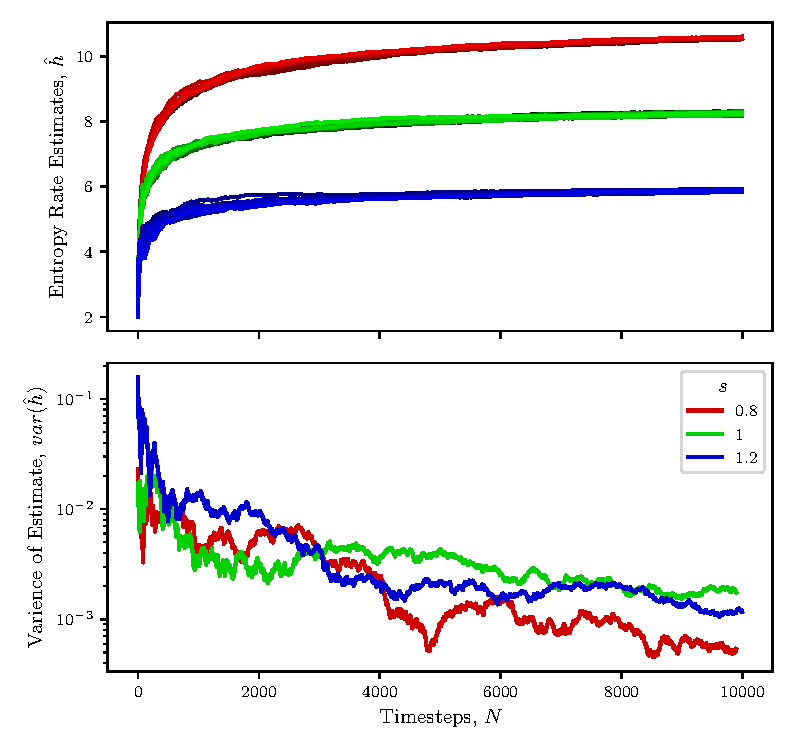
\includegraphics[width=\textwidth]{chapter2/figs/Zipf_entropy_convergence.pdf}
\caption{Convergence of the Kontoyiannis entropy rate estimator on sequences of i.i.d. Zipf distribution realisations with varying Zipf distribution rates, $\alpha$. \label{fig:entropy:zipfconvergence}}
\end{figure}


\autoref{fig:entropy:zipfconvergence} shows the convergence of the estimator for a set of i.i.d. realisations of a Zipf distribution. As discussed in \autoref{sec:textgeneration}, the Zipf distribution is a common tool for generating simple text due to its similarity to the power-law distributions of vocabulary seen in real corpora. The Zipf distribution can be used with a number of scaling parameters, $\alpha$, where larger scaling parameters tighten the distribution, reducing the observed vocabulary size of the sequence and hence the entropy. 

Sequences are generated with 30,000 i.i.d. elements drawn from a Zipf distribution and the entropy rate of estimate of the process is calculated at each timestep between 1 and 30,000 using \autoref{eq:estimate} applied to only the elements before that timestep. Estimates of entropy start very low when few elements are available and rapidly rise as new elements add complexity. Within the first few hundred timesteps entropy estimates can vary between timesteps as new elements are added matching or not-matching previous elements. This is reflected in the high variance between entropies estimates for Zipf process with the same scaling parameter in these early stages. As the number of timesteps included reaches 5000 to 7500 the apparent bias from the asymptotic rate and variance of the estimates are significantly reduced and begin plateauing. 

As more timesteps are added, the estimator continues to converge to the asymptotic entropy and the variance between estimates continues to reduce. High complexity sequences take longer to converge to this entropy, but achieve suitably small levels of bias and variance within 15,000 timesteps even for high entropy sequences. This is an important finding given the speed of calculating these estimates. The algorithm to calculate the match-lengths needed for estimating the entropy is $O(N^3)$ time complexity for the number of included timesteps $N$. As a result, calculations are extremely slow as the number of timesteps gets large. When performing simulations a parsimonious choice of simulation length is advantageous in allowing multiple simulations to be run. Hence, for Zipf distributions a simulation length of 15,000 is deemed sufficient for convergence to the entropy.
%</Zipf convergence>


%<Zipf real entropy>
To confirm the validity of this approach, we can examine the known entropy rate of the Zipf processes. As proved in \autoref{sec:entropyrate}, the entropy rate of an i.i.d. process is simply the entropy of each element. In the case of a Zipf distribution the distribution has entropy\footnote{
	Proof: The probability of a word of rank $k$ being selected from a pool of $V$ elements using scaling parameters $\alpha$ is $(k^\alpha H_{V,\alpha})^{-1}$. Hence, the entropy of each individual element is $\sum_{k=1}^V  (k^\alpha V_{V,\alpha})^{-1} \ln\left( (k^\alpha V_{V,\alpha})^{-1} \right)$. Using $H_{V,\alpha} = \sum_{k=1}^V \frac{1}{k^\alpha}$, this can be rearranged to $\frac{\alpha}{H_{V, \alpha}} \sum_{k=1}^{V} \frac{\ln (k)}{k^{\alpha}}+\ln \left(H_{V, \alpha}\right)$. 
}, 
\begin{equation}
	\frac{s}{H_{V, \alpha}} \sum_{k=1}^{V} \frac{\ln (k)}{k^{\alpha}}+\ln \left(H_{V, \alpha}\right),
\end{equation}
where $H_{V,\alpha}$ is the $V$th generalized harmonic number defined by, 
$$H_{V,\alpha} = \sum_{k=1}^V \frac{1}{k^\alpha},$$
and $V$ is the size of the state space of the Zipf distribution. Many approaches to calculating this entropy use the asymptotic entropy as $V \to \infty$. This draws on the result that $\lim_{V\to \infty} H_{V,s} = \zeta(\alpha)$, where $\zeta$ is the Riemann zeta function. While this asymptotic approach works well for numbers well above 1, the Riemann zeta function diverges to infinity at $\alpha \to 1$. As such, the analytic entropy degenerates as $\alpha \to 1$ and is poorly defined for $\alpha < 1$. In contrast, using a finite choice of $V$ results in well defined processes and entropies for all $\alpha >0$. A choice of $V=199,338$ is made to match the observed total vocabulary size seen in the news-media Twitter data as explored in \autoref{sec:vocabsizes}. For high values of $\alpha$, the two asymptotic and finite entropies are very close (\emph{e.g}, for $\alpha=1.5$ the entropies are 3.18158 and 3.18368 respectively), and only differ significantly as $\alpha$ approaches 1. This finite entropy calculation allows the model to more accurately match the Zipf scaling parameters fitted to real text data, which are often closer to or below~1~\cite{williams_text_2015}.

% <Simulations>
Using simulations of the Zipf process for a variety of values of the scaling parameter $\alpha$, we compare how the estimated entropy rate compares to the `true' entropy rate as calculated above. In \autoref{figs:entropy:convergencetotruth} simulations are run for values of $\alpha$ in the range [0.01, 2] with increments of 0.01. 
High values of $\alpha$ in this range have a progressively lower entropy, as the skewness of the distribution becomes more extreme. This distribution results in a large number of realisations of low rank words creating repeated sequences which lower both the analytic entropy rate and the entropy rate estimate. Values above 2 reduce the entropy rate in vanishingly smaller increments. 

\begin{figure}[!htbp]
\centering
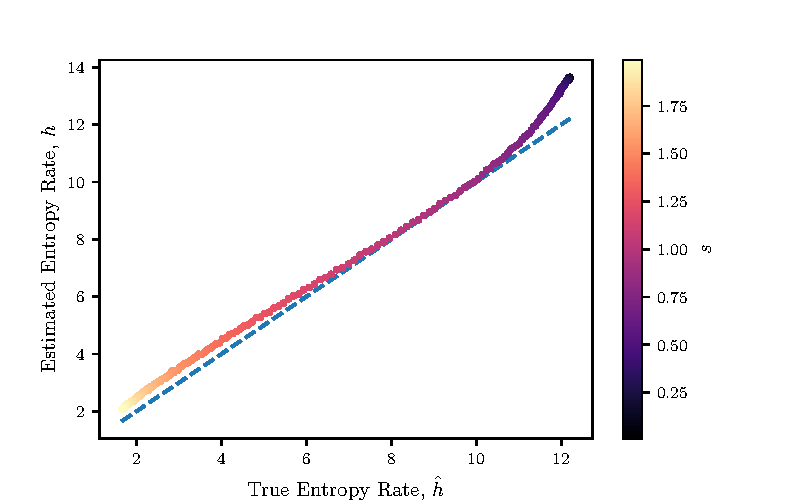
\includegraphics{chapter2/figs/convergence_to_truth.pdf}
\caption{Estimated entropy rates and analytic entropy rates of sequences of 20,000 i.i.d. Zipf distribution random variables with scaling parameter $\alpha$. Dashed line represents the true entropy rate equalling the entropy rate estimate. As values for $\alpha$ approach 0 the high variance of the distributions results in poor estimates due to the finite sample of the Zipf distribution. \label{figs:entropy:convergencetotruth}}
\end{figure}

For values of $\alpha$ between 2 and 0.5, the entropy rate estimate appears to be a rough upper bound on the true entropy rate of the process. This upper bound is only achieved with sufficient lengths of sequences such that the estimator can converge to this upper bound. Indeed, given sufficient length the variance of the estimates on sequences drawn from the same distribution is very low. This is in contrast to the bias of the estimate, which varies with the changing scaling parameter. 

When $\alpha$ becomes lower than 0.5, the Zipf distribution becomes more evenly distributed with reduced skew. This results in a larger probability of low rank word occurrences, producing a process where many words appear very few times. As a result, the finite nature of the sequence results in a entropy rate estimate that grows faster than the true entropy, increasing the bias for these high entropy sequences. 

In general, the convergence of the estimator is sufficient, with a slight caveat: while the estimator convergences to an estimate tightly with very little variance, the bias of the estimate is not constant and varies with the complexity of the sequences. While this finding is itself interesting and warrants future work, the estimator is both consistent and its estimates appear monotonic with the true entropy rate. As such, we will use this estimator to approximate the true entropy rate moving forward, with a cautious eye to the possible effects of this inconsistent bias. 
%</Zipf real entropy>

%<Real data entropy convergence>
To extend from this result, we apply the same approach replacing Zipf distribution generation with text from the news-source Twitter data. 5000 tweets are drawn uniformly from the collection of all tweets from all news-media outlets. These tweets are tokenized and concatenated into a single sequence of natural language text ranging from 85,000 to 90,000 tokens.

Unlike the case of Zipf, we cannot show a true entropy rate for this distribution, as it's unknown, but can demonstrate its convergence.  Each sample has the entropy rate calculated using only the first $N$ tokens, up to the length of 60,000 tokens. \autoref{fig:entropy:realconvergence} shows the clear convergence of the estimator on the real data, approaching an entropy rate of 7.53. As with the Zipf simulations, the variance of the estimated entropy rates of the samples reduces as more tokens are included in the estimate.  The real data takes longer to converge, needing up to 50,000 tokens to achieve a variance of less that $10^{-3}$.

\begin{figure}[!htbp]
\centering
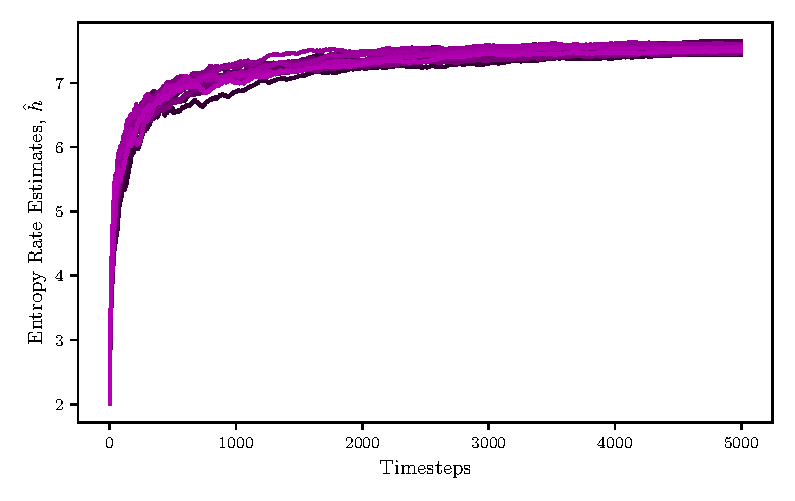
\includegraphics{chapter2/figs/real_entropy_convergence.pdf}
\caption{Convergence of the Kontoyiannis entropy rate estimator on sequences words generated by drawing tweets uniformly without replacement from the pool of all tweets produced by all news-media organisations. Multiple sequences are drawn with most convergence curves overlapping. \label{fig:entropy:realconvergence}}
\end{figure}

%</Real data entropy convergence>

%<Tikz of flow>
\subsubsection{Self entropy rate summary}

\begin{figure}[!htbp]
	\centering
	\includestandalone[width=\textwidth]{chapter2/figs/tikz/self_flow}
	\caption{A conceptual diagram of entropy rate estimation using the Kontoyiannis entropy rate estimation. Tweets shown as blue rectangles are positioned in time and contain textual content. Content proceeding the position \emph{Now} will have snippets of text matched with text from the history of the process, denoted by {\color{orange}orange} and \underline{underlined} text. These text matches are used to calculate $\Lambda_i$ which is used in the entropy estimate. \label{fig:entropy:selfflow}} 
\end{figure}

Before moving away from the entropy rate of a single process, we visualise the how the Kontoyiannis entropy rate estimator works for real data. \autoref{fig:entropy:selfflow} shows a simplified version of the conceptual entropy rate calculation. For a given Twitter user, tweets appear sequentially, separated in time. At any given time, the content of the immediate future of that user's tweets is compared to the entire history of the tweets before that time. This process is then repeated for all possible times in the data. In essence, the calculation of the $\Lambda_i$ is a repeated examination of how much of the immediate complexity at timestep $i$ can be described using the history of the sequence. In total, this estimator provides an average of how many bits are needed to describe the future of this process given its past at any point. 

%% Histogram of self entropy rates ??

%</Tikz of flow>

\section{Cross entropy rate}

To create a notion of information flow, we need to move beyond looking at an individual source in isolation. To do so, we need a tool of comparison between sources rooted in our tools from information theory. We find such a tool in a generalisation to a Kontoyiannis cross entropy rate.

Similar to the extension of entropy, $$H(X) = \sum_{x \in \mathcal{X}} p(x)\log p(x)=-\mathbb{E}[\log P(X)],$$ to cross entropy, $$H(p,q) = \sum_{x \in \mathcal{X}} p(x)\log q(x) = -\mathbb{E}_p[\log q(X)],$$  in \autoref{def:crossentropy}, we can generalise our notion of Kontoyiannis entropy rate from \autoref{def:Kontoyiannis} to a \emph{cross} entropy rate which we will call the Kontoyiannis cross entropy rate. This Kontoyiannis cross entropy rate comes in two forms, a full cross entropy and a time-synced cross entropy.

\begin{definition}[Kontoyiannis Full Cross Entropy Rate]
	The cross entropy rate of a {\color{target} target process} $\mathcal{T}$ coded from a {\color{source} source process} $\mathcal{S}$ can be estimated via,
	\begin{equation}
	H(\mathcal{T} || \mathcal{S})=\frac{N_{\mathcal{T}} \log _{2} N_{\mathcal{S}}}{\sum_{i=1}^{N_{\mathcal{T}}} \Lambda_{i}(\mathcal{T}| \mathcal{S})}
	\end{equation}
	Where $N_{\mathcal{X}}$ is the length of process $\mathcal{X} \in \{\mathcal{T}, \mathcal{S}\}$ and $\Lambda_{i}(\mathcal{T}| \mathcal{S})$ is given by the shortest subsequence starting at position $i$ in the {\color{target}target} $\mathcal{T}$ that does not appear as a contiguous subsequence anywhere in the {\color{source}source} $\mathcal{S}$.
	\begin{equation}
	\Lambda_{i}(\mathcal{T}| \mathcal{S}) = \max \left\{\ell: T_i^{i+\ell}=S_{j}^{j+\ell}, 0 \leq j \leq N_{\mathcal{S}},  0 \leq \ell \leq \min( N_{\mathcal{S}}- j , N_{\mathcal{T}}- i )\right\},
	\end{equation}
	where $T_a^{b}$ and $S_a^b$ are continuous subsequences starting from index $a$ to index $b$ of the {\color{target} target}, $\mathcal{T}$, and  {\color{source} source}, $\mathcal{S}$, processes respectively.
\end{definition}

This approach to cross entropy matches segments of text in the {\color{target}target} to segments of text anywhere in the {\color{source}source} in the same manner that the Kontoyiannis entropy rate matched segments of text in the future of a process from a index, $i$, to the history before the index. In contrast to the entropy rate estimate, which asked how much information was needed on average to \emph{describe the future of a source from its past}, this cross entropy rate estimate is asking how much information is needed on average to \emph{describe the target given full knowledge of the source}. 

\begin{figure}[!htbp]
	\centering
	\includestandalone[width=\textwidth]{chapter2/figs/tikz/unsynced_flow}
	\caption{A conceptual diagram of Kontoyiannis full cross entropy rate estimation. Tweets shown as rectangles are positioned in time for both a target and source, containing textual information. Content in the {\color{source}source} is matched with content in the immediate future of the {\color{target}target} for a given time point, $t$, to calculate match-lengths. This time point is shifted along the {\color{target}target} timeline to average match-lengths and calculate the full cross entropy rate.\label{fig:entropy:unsyncedflow}} 
\end{figure}

This full knowledge over all of the process gives the estimator the `Full' in its title, but presents a impropriety. In the context of our problem, this estimator is cheating by viewing the future of news through the lens of the source process. 

As \autoref{fig:entropy:unsyncedflow} illustrates, the text subsequence match in the target could be drawn from future time points in the source. Restated, the cross entropy rate will, in-part, be describing how much information is needed to encode the future of a piece of target news already knowing the future of the news from another source. While this may be an interesting insight in itself, and could be used in future work to format a notion of information divergence, it doesn't probe the underlying process of \emph{information flow} with which this thesis focuses. 

Rather than looking at the entire lifetime of the source during the matching calculations, we can reduce our search space to the text that occurred in the \emph{past} of the source. To achieve this we use an important piece of our data, the time that tweets occurred. For each word in the target process, $T_i$ has an associated time with it, $t(T_i)$. When matching the future of $\mathcal{T}$, starting from an index $i$, we can reduce the source process, $\mathcal{S}$ to only the words that were themselves tweeted before time $t(T_i)$. 

Put simply, we can alter the Kontoyiannis full cross entropy rate to a time-synced cross entropy rate by replacing the full source process, $\mathcal{S}$, with a time reduced source process $\mathcal{S}_{ \leq t(T_i)}$. This can be seen visually in \autoref{fig:entropy:timesyncedflow} and is formally defined as follows.

\begin{definition}[Kontoyiannis Time-synced Cross Entropy Rate]
	The time-synced cross entropy rate of a {\color{target}target} process $\mathcal{T}$ coded from a {\color{source}source} process $\mathcal{S}$ can be estimated via,
	\begin{equation}
	H(\mathcal{T} || \mathcal{S})=\frac{N_{\mathcal{T}} \log _{2} N_{\mathcal{S}}}{\sum_{i=1}^{N_{\mathcal{T}}} \Lambda_{i}(\mathcal{T}| \mathcal{S}_{\leq t(T_i) } )}
	\end{equation}
	Where $\Lambda_{i}(\mathcal{T}| \mathcal{S}_{\leq t(T_i) })$ is given by the shortest subsequence starting at position $i$ in {\color{target}target} $\mathcal{T}$ that does not appear as a contiguous subsequence in the time reduced {\color{source}source} $\mathcal{S}_{\leq t(T_i) }$ where,
	\begin{equation}
	\mathcal{S}_{\leq t(T_i) } = \{S_j | t(S_j) \leq t(T_i),  \forall i \}.
	\end{equation}
	Which gives,
	\begin{align*}
	\Lambda_{i}(\mathcal{T}| \mathcal{S}_{\leq t(T_i)}) = \max \{\ell: T_i^{i+\ell}=S_{j}^{j+\ell}, 0 \leq j \leq N_{\mathcal{S}},  \\  0 \leq \ell \leq \min( N_{\mathcal{S}}- j , N_{\mathcal{T}}- i ) \},
	\end{align*}
	where $T_a^{b}$ and $S_a^b$ are continuous subsequences starting from index $a$ to index $b$ of the {\color{target} target}, $\mathcal{T}$ process, and the time reduced {\color{source} source}, $\mathcal{S}_{\leq t(T_i)}$, respectively.
\end{definition}

\begin{figure}[!htbp]
	\centering
	\includestandalone[width=\textwidth]{chapter2/figs/tikz/timesynced_flow}
	\caption{A conceptual diagram of Kontoyiannis time-synced cross entropy rate estimation. Tweets shown as rectangles are positioned in time for both a target and source, containing textual information. Content in the {\color{source}source} that occurs before time $t$ is matched with content in the immediate future of the {\color{target}target} from $t$ to calculate match-lengths. This time point is shifted along the {\color{target}target} timeline to average match-lengths and calculate the time-synced cross entropy rate.\label{fig:entropy:timesyncedflow}} 
\end{figure}


% Informantion flow idea
This time-synced cross entropy rate is testing not just the differences in the language processes of the source and target, but also measuring what information in the target is present in the source's history. This is an important distinction, as it allows us to probe a very important aspect of our data, namely, the time in which news is created. 

If a piece of information appears earlier in the source than in the target, it will be detected during the match length search, resulting in a lower entropy. This is to say, in the context of news, if the {\color{source}source} breaks a story first, \emph{less} information is required to describe the subsequent news output from the {\color{target}target}. 

Conversely, if a {\color{target}target} produces a piece of information before the {\color{source}source}, then that information will not appear in the history of the time-synced source during the match-length search. This will result in lower values of $\Lambda_i$ for that piece of information, which raises the cross entropy rate.

From this, we can find that, on average, if a {\color{source}source} produces information earlier than a {\color{target}target}, the cross entropy rate, $\hat{h}(\mathcal{T} || \mathcal{S})$, will be lower than if the {\color{target}target} produces information earlier than the {\color{source}source}. This method of examining who produces information first can be extended into a notion of \emph{information flow}, a discussion we will leave for \autoref{ch:quotermodel}.


\subsection{Validating the assumptions of cross entropy estimation}

To validate these new cross entropy rate estimators a similar process is performed as with the entropy rate. Fortunately, many of the assumptions transfer over directly.

In the case of ergodicity, stationarity and the Doeblin Condition, all three are properties of the process under investigation, which we argued above are well founded. We introduce an additional condition on the processes for the sake of cross entropy rates, namely that the processes have the same state space. This additional condition extends the earlier conditions to apply jointly between both the source and target processes. While not all news-media organisations will have the same realisations of words in their corpus, the processes could be reasonably thought to have the same state space, as all processes are using English and discussing similar topics.

This then leads naturally to the next question of convergence. Following a similar process of uniform withdrawals from a distribution will result in functionally similar convergence to the entropy rate above. Indeed, this can be seen in \autoref{fig:entropy:realcrossconvergence}, where tweets are draw uniformly from the pool of all tweets and cross entropy rates are calculated on the resulting sequences. Here, the cross entropy rate is denoted $\hat{h}_{\times}$ to distinguish from the entropy rate estimates $\hat{h}$. This figure is, as expected, functionally similar to \autoref{fig:entropy:realconvergence} from the entropy rate section above. This cross entropy rate calculation is fundamentally no different from the original entropy rate calculation with these sequences, as a randomly selected history of another process is just a useful and a randomly selected history the original process when both draw from the same distribution.


\begin{figure}[!htbp]
	\centering
	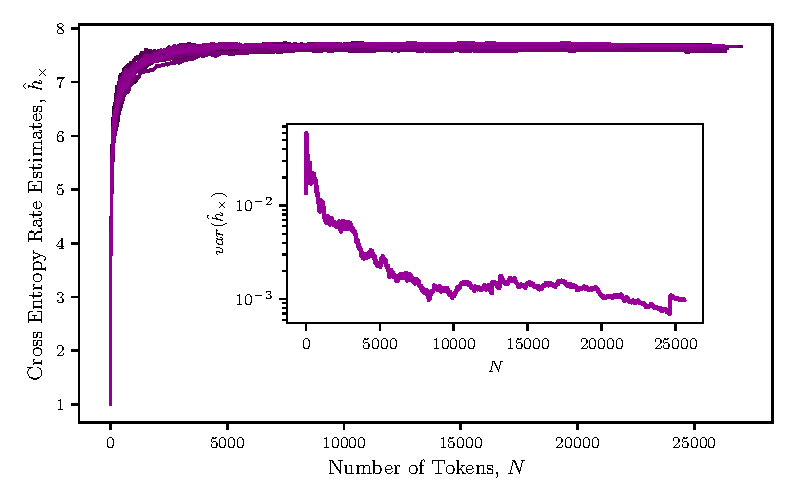
\includegraphics{chapter2/figs/cross_real_entropy_convergence}
	\caption{Convergence of the Kontoyiannis time-synced cross entropy rate estimator on pairs of sequences independently generated by drawing tweets uniformly without replacement from the pool of all tweets produced by all news-media organisations.} \label{fig:entropy:realcrossconvergence}
\end{figure}

A more nuanced investigation of the cross entropy convergence emerges when we utilise processes with \emph{different} distributions. \autoref{fig:entropy:zipfcrossconvergence} does exactly this. Using pairs of scaling parameters for different Zipf distributions, simulations of 30,000 long i.i.d.~ processes are made with separate target and source processes. The cross entropies rates are then estimated across these pairs. When the scaling parameters are equal, $\alpha_{source}=\alpha_{target}$, we observe the same entropy and convergence pattern as we would for a single i.i.d. process with that distribution. 

\begin{figure}[!htbp]
	\centering
	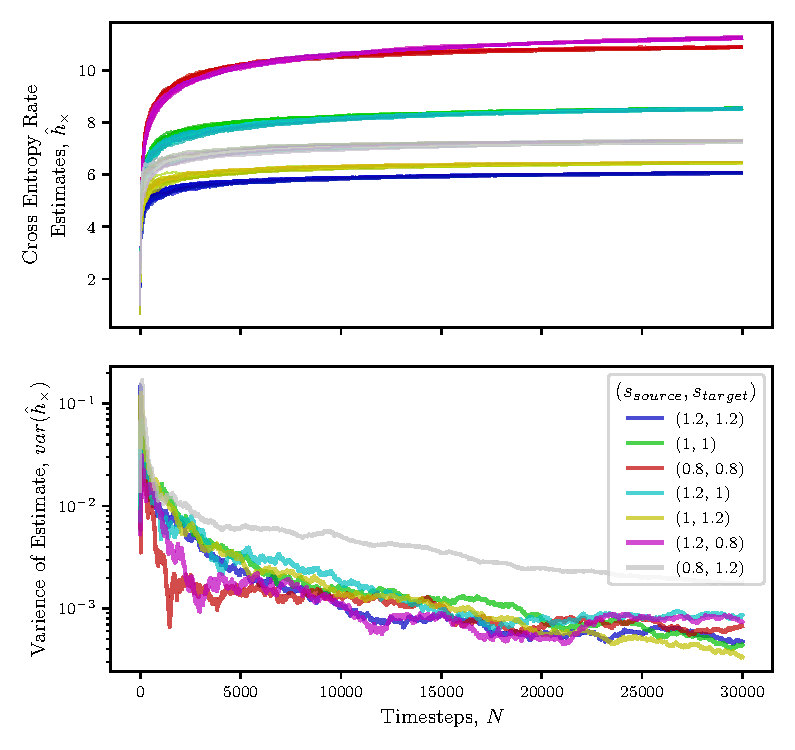
\includegraphics{chapter2/figs/cross_Zipf_entropy_convergence.pdf}
	\caption{Convergence of the Kontoyiannis time-synced cross entropy rate estimator on pairs sequences of i.i.d. Zipf distribution realisations with varying pairs of Zipf distribution rates, $\alpha_{source}$ and $\alpha_{target}$. } \label{fig:entropy:zipfcrossconvergence}
\end{figure}

When $\alpha_{source} \neq \alpha_{target}$ the entropy rates vary, and are not always similar to the entropy rate of the target or the source. Most cross entropy rates converge at a similar pace to the entropy rates above, although large deviations between distributions can reduce this rate of convergence. In particular when the source has significantly higher complexity than the target, as in the case of $(\alpha_{source}, \alpha_{target}) = (0.8,1.2)$, the entropy takes much longer to converge as it requires longer for common patterns to occur in the high complexity source for sequence matching. % talk more





\subsection{Predictability}
With the Kontoyiannis cross entropy rate estimator converging, we also want to generalise the notion of maximal predictability.
We introduced maximal predictability, $\pi^{max}(S,V)$,  in \autoref{def:maximialpredictability} as it is a robust way of determining an upper bound on how well the future of a process could be predicted from its past. The use of the state space size, allows for normalisation of the entropy rate when state spaces are large. The state space size will be represented as $V$ as the state space of language is the vocabulary.

In order to generalise this notion of maximal predictability, we need to identify the two replacements for the inputs. The replacement for entropy rate is trivially the cross entropy rate, but the choice of state space size is more nuanced. Three choices are possible, the state space of the source, $V_{source}$, the target, $V_{target}$, and the union of the state spaces $V_{union}$. 

The original motivation behind the maximal predictability is to normalised the entropy by \emph{how complex the system we are trying to predict is}. This complexity is a property of the target. While a complex source does change how well the target can be predicted, it is the property of the target that needs to be controlled for. As such, the choice of $V_{target}$ is taken and referred to as simply $V$ in the following definition.

\begin{definition}[Maximal Cross Predictability]
For two processes $S$ and $T$ with cross entropy $H(T||S)$ from the source to the target and state space size $V$ of the target, the maximal cross predictability, $\pi^{max}(T||S)$ can be found numerically by solving, 
\begin{equation}
H(T||S)  = H(\pi^{max}(T||S)) + (1 - \pi^{max}(T||S)) \log (V - 1),
\end{equation}
for $\pi^{max}(T||S)$.
\end{definition}


\subsection{A note on package development}

As stated earlier, a key challenge in estimating these Kontoyiannis cross entropy rates is calculation speed. With time complexities of $O(N^3)$ on the number of input tokens, efficient code is necessary to allow for estimation using long sequences. To achieve speed and contribute to this field of work more broadly, a speed-focused open source package was developed to help researchers efficiently and easily calculate entropy rates such as those discussed above. The important snippets from code contributions of the package, named `ProcessEntropy', are available in \autoref{app:code} and this section will outline tools used in speeding the code up.

Fundamental complexity limitations of the subsequence matching algorithm mean that speed improvements need to come from smart implementation. Two techniques used are interesting enough to discuss briefly here, hashing and just-in-time compilation.

In the context of analysing language like a process, each word is simply an element of the state space. As such, each word can be assigned a unique number to represent its position in the state space. In doing so it allows the computations of the $\Lambda_i$'s to be performed using much faster integer operations. In the ProcessEntropy package, words are converted to 32 bit unsigned integers using Fowler–Noll–Vo hashing. Fowler–Noll–Vo is a non-cryptographic hash function which is fast to compute. This converts words to the same integer every time, with no collisions. 


The second major speed improvement is drawn from the use of just-in-time (JIT) compilation. Python is commonly used in scientific settings as an interpreted language. In most contexts the Python interpreter allows variables to exist as dynamic types. As such, the exact same function can often be applied to integers, strings or other objects interchangeably. As a result, a larger number of type checks and other control operations are required during runtime, slowing down computation. JIT compilers such as Numba\footnote{\url{https://numba.pydata.org/}} operate by observing variable types at the start of runtime and generating optimized machine code. 

\begin{figure}[!htbp]
\centering
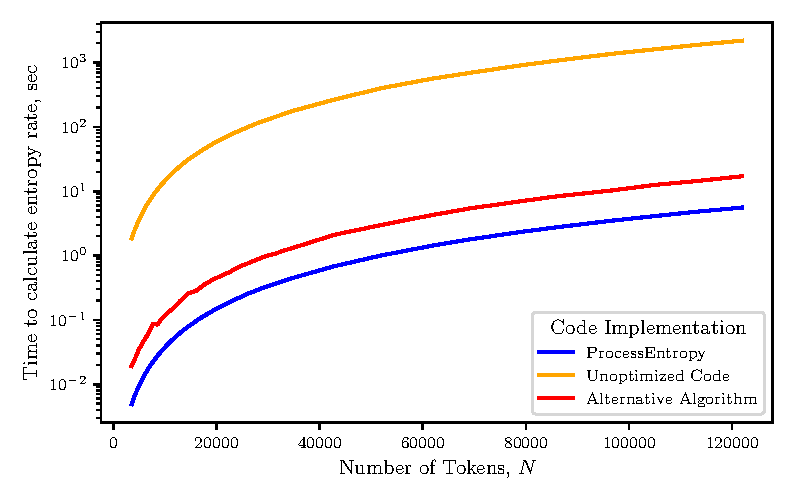
\includegraphics{chapter2/figs/speedcomparison.pdf}
\caption{A speed comparison of implementations of the Kontoyiannis entropy rate estimator. ProcessEntropy uses code from the package of the same name, unoptimized code is the same algorithm as ProcessEntropy without type and compile optimizations and Alternative Algorithm is an optimized alternative algorithm using the built-in \texttt{.contains()} method from the \texttt{stringlib} library. \label{fig:entropy:speedcomparison}}
\end{figure}


\autoref{fig:entropy:speedcomparison} shows a comparison of the optimized methods compared to alternatives. The ProcessEntropy package consistently performs the fastest, using the speed improvements listed above and efficient implementation. In contrast, the unoptimized code (written in pure Python without fixed type compiling or parallelisation) performs over two orders of magnitude slower for all input sizes. For comparison, an alternative algorithm is shown using the highly optimized \texttt{.contains()} method included in the \texttt{stringlib} library from Cython. This method uses a simplified version of the Boyer-Moore string-search algorithm, incorporating ideas from Horspool and Sunday~\cite{lundh_stringlib_2006}. Even with the alternative algorithm written in C, the ProcessEntropy code outperforms consistently. The package is available on the Python Package Index (PyPi) for interested researchers\footnote{\url{https://pypi.org/project/ProcessEntropy/}}.

\subsection{Running estimations}\label{sec:running_estimations}

To close this chapter, the tools developed throughout can now be applied to the news dataset introduced in \autoref{ch:data}. This news data contains 154 year-long Twitter content streams, with mean of 337,284 tokens. %
%(min 8059, max 2,627,305, $\sigma=$377,994)
Each stream has its entropy rate calculated and each pair of news-media outlets have their time-synced cross entropy rate calculated in both directions. In total this is 23,716 entropy rate estimations on these long sources. Even, with the efficient ProcessEntropy package, these calculations take well over a week, and this analysis would not be computationally tractable on the available hardware using the other implementations of the code.


\begin{figure}[!htbp]
	\centering
	\begin{subfigure}[t]{0.58\textwidth}
		\centering
		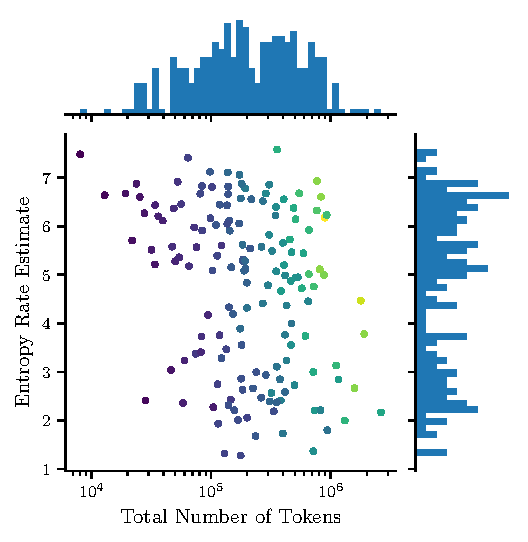
\includegraphics{chapter2/figs/tokens_vs_self_entropy_rate.pdf}
		\caption{}
	\end{subfigure}
	~
	\begin{subfigure}[t]{0.38\textwidth}
		\centering
		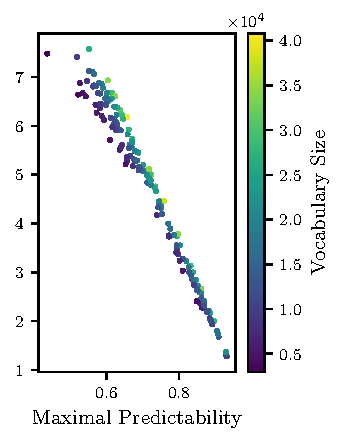
\includegraphics{chapter2/figs/entropy_vs_predictability.pdf}
		\caption{}
	\end{subfigure}
	\caption{Entropy rate estimates for the Twitter timelines of 154 news-media organisations during the calendar year of 2019. (a) shows the limited relationship between the total number of tokens in the Twitter text history and the entropy rate estimates. (b) shows the tight relationship between the entropy rates estimate and its derived maximal predictability, with higher variances seen at high entropies.}
	\label{fig:entropy:selfentropyrateestimates}
\end{figure}

\autoref{fig:entropy:selfentropyrateestimates} shows these entropy rate estimates on the news-media Twitter histories. Importantly, the entropy rate estimate shows very limited correlation with the total length of the content (number of tokens) or with the vocabulary size. This indicates that the estimate entropy rates have converged. Further, we see an expected strong correlation between the entropy rate estimate and the maximal predictability. Notably, the variance between the two increases for higher entropy rates, where larger vocabulary sizes can have an outsized effects on estimates. 

\begin{figure}[!htbp]
\centering
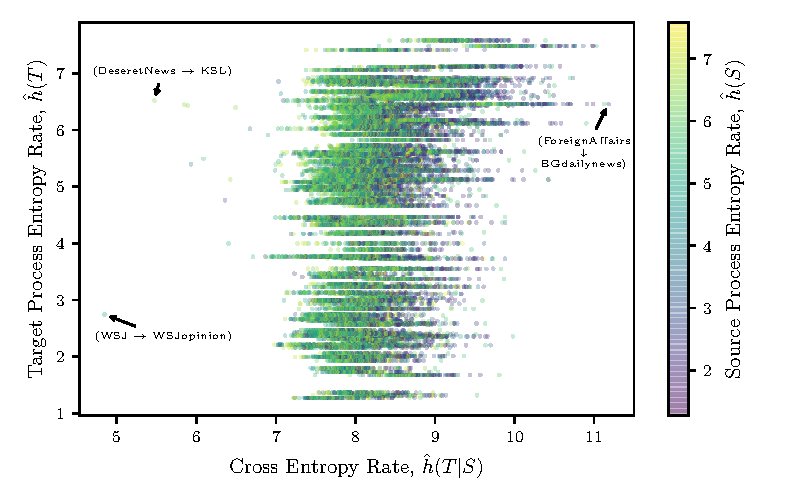
\includegraphics{chapter2/figs/cross_vs_self_entropy_rates.pdf}
\caption{Time-synced cross entropy rate estimates on pairs of news-media organisations on Twitter using their full content for the 2019 calendar year. Cross entropy rates are compared to the entropy rate estimates of the sources, $S$, and targets, $T$, in isolation. Example outliers are shown as `(source $\to$ target)'.} \label{fig:entropy:crossentropyestimates}
\end{figure}

Following this, the time-synced cross entropy rates are estimated and shown in \autoref{fig:entropy:crossentropyestimates}. Here we see similar results. The target entropy rate has limited correlation with the cross entropy rate ($R^2=0.116$), except for very high entropy targets, which receive higher cross entropy rates due to the high complexity nature of the target information. In contrast, source entropy rate has almost no correlation with the cross entropy rate ($R^2=0.0497$).

Several outliers exist at both the high and low ends of cross entropy. Low cross entropy outliers are all pairs of news-media organisations which are deeply related. Two examples of this are (\emph{@WSJ} $\to$ \emph{@WSJopinion}), where the information in the \emph{Wall Street Journal's} Opinion news stream can be described extremely efficiently by the \emph{Wall Street Journal's} main news stream, and (\emph{@DeseretNews} $\to$ \emph{@KSL}), where both news-media organisations report news specifically about Salt Lake City, Utah, and \emph{Deseret News} previously owned and remains closely linked to \emph{KSL}. 

At the high end of the cross entropy, pairs of organisations tend to have very little relationship. The highest cross entropy rate pair is (\emph{@ForeignAffairs} $\to$ \emph{@BGdailynews}) which suggests that very little information from the international relations focused \emph{Foreign Affairs Magazine} is useful in describing `Southcentral Kentucky's No. 1 Source for Information' \emph{Bowling Green Daily News}.

In total, the cross entropy rates are much higher than the entropy rates, highlighted in \autoref{fig:entropy:estimatedesnities}. This is an expected behaviour, as predicting the language and content behaviour of someone else is naturally harder than predicting your own future text. These distributional differences are carried over into maximal predictability, with generally lower maximal cross predictabilities.

\begin{figure}[!htbp]
	\centering
	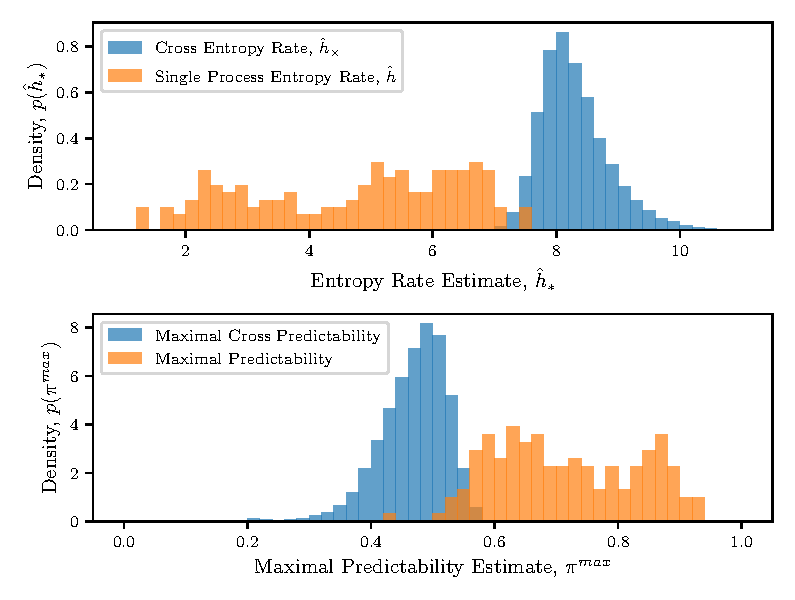
\includegraphics{chapter2/figs/entropy_densities.pdf}
	\caption{Comparison of cross and individual measures of information complexity. Self entropy rates and self maximal predictabilities are calculated for each of the 154 news-media organisations. Cross entropy rates and cross maximal predictabilities are calculated for all pairs of organisations. The distribution of the cross information and self information estimates are compared.
	Cross entropy rates are higher than self entropy rates as news-media organisations, in general, do not contain information in their history that is more useful to other news-media organisations than it is to themselves. This is reflected in the lower maximal cross predictabilities.  } \label{fig:entropy:estimatedesnities}
\end{figure}

\subsubsection{Concluding remarks}
Using both the Kontoyiannis entropy rate estimate and the generalised Kontoyiannis cross entropy rate estimate, we can construct a set of summary statistics about the language and behaviour patterns of the news sources under investigation and their relationships. These estimators are well founded on both a theoretical backbone and experimental evidence, and can be applied efficiently using the new open-source package, ProcessEntropy. From here, these calculated estimates can be used to extract the measures of information flow sought in this thesis, a task for \autoref{ch:quotermodel}.



